% =============================================================================
% Soutenance préfinale — Fil rouge
% Gestion conjointe et coordonnée : bloc opératoire / lits / ambulatoire.
%
% Fusionne les supports :
%   - soutenance/Kaua_SMA_9_octobre.tex          (SMA, simulation, résultats)
%   - rapport_jupyter_notebook_LIRE_ALEA/slide_avancement_v2.tex
%   - soutenance/Soutenance_intermediaire.tex     (sections 1-8, workflow)
%   - rapport_jupyter_notebook_LIRE_ALEA/RAPPORT.md (benchmark 10 méthodes)
%
% Thème Mid-Century Modern, palette Kraft (comme Soutenance_intermediaire.tex).
%
% Organisation : ce master n'assemble que les inputs ; le contenu de chaque
% partie vit dans sections/ (01_introduction ... 08_conclusion). La section
% KYST est importee depuis ../thomas.tex, juste avant la conclusion.
%
% Compilation (LuaLaTeX requis par le thème), depuis soutenance/prefinal/ :
%   lualatex Soutenance_prefinal.tex
%   biber    Soutenance_prefinal
%   lualatex Soutenance_prefinal.tex
%   lualatex Soutenance_prefinal.tex
% =============================================================================
\documentclass[aspectratio=169,11pt]{beamer}
\usepackage{../beamerthememidcenturymodern}
\mcmTheme{Kraft}

% Palette Kraft reprise de Kaua_SMA_9_octobre.tex (frames importées telles quelles).
\definecolor{McmTerracotta}{HTML}{9C4732}
\definecolor{McmSage}{HTML}{6B7F3A}
\definecolor{McmAmber}{HTML}{DB6720}
\definecolor{McmWarm}{HTML}{F8F6F2}
\definecolor{McmSand}{HTML}{E8D5B5}
\definecolor{McmInk}{HTML}{1A1A1A}
\definecolor{McmMuted}{HTML}{5A534E}

\usepackage[french]{babel}
\usepackage{amsmath,amssymb}
\usepackage{booktabs}
\usepackage{tikz}
\usetikzlibrary{arrows.meta,positioning,calc,babel,backgrounds,fit}
\usepackage{graphicx}
\usepackage{qrcode}
\graphicspath{{../figures/}{../../rapport_jupyter_notebook_LIRE_ALEA/figures/}}
\usepackage[backend=biber,style=authoryear,sorting=nyt]{biblatex}
\addbibresource{../Etatdelart.bib}

\AtEveryCite{\color{mcmPrimary}}

% Note de source sous les frames.
\newcommand{\source}[1]{\par\vspace{4pt}{\color{mcmBlack!60}\tiny #1}}

% Transition de section : sommaire courant.
\AtBeginSection[]{%
  \begin{frame}{Sommaire}
    \tableofcontents[currentsection]
  \end{frame}
}

% ----------------------------------------------------------------------------
% Métadonnées
% ----------------------------------------------------------------------------
\title[Bloc, lits \& ambulatoire]{Optimisation conjointe du bloc opératoire,
  des lits d'hospitalisation et de l'ambulatoire}
\subtitle{Soutenance préfinale --- du planning statique au planning robuste}
\author[IA \& Santé --- Groupe 2]{IA et Santé --- Groupe 2}
\date{Soutenance préfinale --- 2026}

\begin{document}

% =============================================================================
% PAGE DE TITRE ET SOMMAIRE
% =============================================================================
\begin{frame}
  \titlepage
\end{frame}

\begin{frame}{Sommaire}
  \tableofcontents
\end{frame}

% =============================================================================
\section{Introduction et contexte}
% =============================================================================

% Les trois ressources du fil rouge et leur interdépendance.
\begin{frame}{Le bloc opératoire : des ressources rares et couplées}
  \small
  \begin{columns}[T,onlytextwidth]
    \begin{column}{0.31\textwidth}
      \begin{exampleblock}{\centering Bloc opératoire}
        \centering\footnotesize
        Salles, vacations de 4\,h\\
        Chirurgien, équipe d'anesthésie\\
        Temps opératoire contraint
      \end{exampleblock}
    \end{column}
    \begin{column}{0.31\textwidth}
      \begin{block}{\centering Lits d'hospitalisation}
        \centering\footnotesize
        Capacité limitée ($\sim$45 lits)\\
        Séjours de plusieurs jours\\
        Pics et creux d'occupation
      \end{block}
    \end{column}
    \begin{column}{0.31\textwidth}
      \begin{alertblock}{\centering Places ambulatoires}
        \centering\footnotesize
        Séjours courts\\
        Forte sensibilité à l'heure\\
        Ressource distincte des lits
      \end{alertblock}
    \end{column}
  \end{columns}

  \vspace{0.35cm}
  \begin{alertblock}{Le constat}
    \small Ces décisions sont \textbf{interdépendantes} : un lit non disponible
    annule une opération, une place ambulatoire saturée bloque la sortie de
    salle, une salle fermée déplace toute la journée. Pourtant, ces ressources
    sont le plus souvent \textbf{pilotées séparément}.
  \end{alertblock}
  \source{Dimensionnement clinique : $\sim$45 lits classiques et 21 lits
    ambulatoires (consignes du fil rouge).}
\end{frame}

% Le glissement de logique : flux poussé -> flux tiré.
\begin{frame}{Du flux poussé au flux tiré}
  \small
  \begin{columns}[T]
    \begin{column}{0.48\textwidth}
      \begin{block}{Organisation actuelle : flux poussé}
        \begin{itemize}
          \item Le chirurgien choisit une date selon son planning.
          \item Blocs, lits et équipes s'adaptent ensuite.
          \item Résultat : pics et creux d'activité.
        \end{itemize}
      \end{block}
    \end{column}
    \begin{column}{0.48\textwidth}
      \begin{block}{Approche proposée : flux tiré}
        \begin{itemize}
          \item La date dépend des ressources disponibles.
          \item Bloc et lits sont optimisés conjointement.
          \item Le chirurgien choisit parmi deux propositions.
        \end{itemize}
      \end{block}
    \end{column}
  \end{columns}

  \vspace{0.2cm}
  \begin{alertblock}{Idée centrale du projet}
    Optimiser \textbf{simultanément} le bloc, les lits et l'ambulatoire, et
    proposer au praticien une \textbf{Date A} (optimale) et une
    \textbf{Date B} (alternative).
  \end{alertblock}
  \source{Le chirurgien conserve la décision finale : l'outil est une aide à la
    décision, pas un automate.}
\end{frame}


% =============================================================================
\section{Problématique}
% =============================================================================

\begin{frame}{Problématique : objectifs, contraintes et difficultés}
  \footnotesize
  \begin{columns}[T,onlytextwidth]
    \begin{column}{0.48\textwidth}
      \begin{block}{Objectif}
        Affecter chaque patient à une \textbf{vacation} compatible avec sa
        spécialité et à un \textbf{lit}, pour :
        \begin{itemize}
          \item occuper le bloc sans dépasser les vacations ;
          \item lisser les lits et les places ambulatoires ;
          \item réserver une marge pour les urgences.
        \end{itemize}
      \end{block}
      \begin{block}{Contraintes}
        \begin{itemize}
          \item \textbf{Médicales} : spécialité, urgence ;
          \item \textbf{Organisationnelles} : chirurgien, équipes ;
          \item \textbf{Temporelles} : jour, horaires, séjour.
        \end{itemize}
      \end{block}
    \end{column}
    \begin{column}{0.48\textwidth}
      \begin{alertblock}{Difficultés}
        \begin{itemize}
          \item \textbf{Combinatoire élevée} : le produit des affectations
            explose.
          \item \textbf{Multi-critères} : bloc, lits et ambulatoire
            s'opposent.
          \item \textbf{Dépendances fortes} : le bloc retentit sur les lits
            plusieurs jours après.
        \end{itemize}
      \end{alertblock}
      \begin{center}
        Problème d'affectation sous contraintes : \textbf{NP-difficile}.
      \end{center}
    \end{column}
  \end{columns}
  \source{Formulation : affectation patient $\rightarrow$ salle $\rightarrow$
    jour (variables $x_{i,s,t}$).}
\end{frame}


% =============================================================================
\section{Modélisation et approche statique}
% =============================================================================

% Ensembles, paramètres et variables.
\begin{frame}{Ce qu'il faut décider : variables et paramètres}
  \small
  \begin{columns}[T,onlytextwidth]
    \begin{column}{0.52\textwidth}
      \begin{block}{Ensembles et décision}
        \begin{tabular}{@{}ll@{}}
          $P = \{1,\dots,n\}$ & patients à planifier \\
          $S = \{1,\dots,m\}$ & salles opératoires \\
          $T = \{1,\dots,H\}$ & jours de l'horizon \\
          $x_{i,s,t} \in \{0,1\}$ & patient $i$ en salle $s$ le jour $t$ \\
        \end{tabular}
        \vspace{4pt}
        \[
          \sum_{s \in S}\sum_{t \in T} x_{i,s,t} = 1
          \quad \forall i \in P
        \]
      \end{block}
    \end{column}
    \begin{column}{0.46\textwidth}
      \begin{block}{Paramètres issus des données}
        \begin{tabular}{@{}ll@{}}
          $d_i$ & durée opératoire du patient $i$ \\
          $S_i$ & durée de séjour (jours) \\
          $a_i$ & ambulatoire ($1$) ou non ($0$) \\
          $C_{\text{vac}}$ & capacité d'une vacation \\
          $L_{\max}$ & capacité en lits \\
          $A_{\max}$ & capacité en places ambu. \\
          $\tau_{\text{Urg}}(t)$ & marge urgences du jour $t$ \\
        \end{tabular}
      \end{block}
    \end{column}
  \end{columns}
  \source{Durées $d_i$ et $S_i$ estimées à partir de l'historique ; capacité de
    vacation typique : 4\,h (240 min).}
\end{frame}

% Fonction objectif : trois tensions.
\begin{frame}{Fonction objectif : trois tensions à équilibrer}
  \footnotesize
  \[
    \begin{aligned}
      \min\; & \alpha \sum_{J \in T}\bigl(L(J)-L_{\text{cible}}(J)\bigr)^2
             + \beta \sum_{J \in T}\bigl(A(J)-A_{\text{cible}}(J)\bigr)^2 \\
             & + \gamma \sum_{J \in T}\Delta_{\text{bloc}}(J)^2
    \end{aligned}
  \]
  \begin{columns}[T,onlytextwidth]
    \begin{column}{0.52\textwidth}
      \begin{block}{Lecture}
        \begin{itemize}
          \item terme 1 : pénalise les \textbf{pics et creux} de lits ;
          \item terme 2 : lisse la charge des \textbf{places ambulatoires} ;
          \item terme 3 : pénalise l'écart à la capacité du bloc, urgences
            comprises ;
          \item $\alpha,\beta,\gamma>0$ : poids à régler.
        \end{itemize}
      \end{block}
    \end{column}
    \begin{column}{0.46\textwidth}
      \begin{alertblock}{Coût réellement implémenté}
        \footnotesize
        \[
          \begin{aligned}
            \text{coût} &= 5 \cdot \text{dépassement}_{\text{vac}}
                          + 3 \cdot \text{dépassement}_{\text{lits}} \\
                         &\quad + 0{,}05 \cdot \text{écart-type}_{\text{vac}}
          \end{aligned}
        \]
        La \textbf{fitness} vaut $-\text{coût}$ : on maximise, $0$ = planning
        parfaitement faisable et équilibré.
      \end{alertblock}
    \end{column}
  \end{columns}
  \source{Le terme bloc et le terme lits sont des contraintes dures relâchées ;
    l'ambulatoire intervient dans la formulation cible et via le type de prise
    en charge prédit.}
\end{frame}

% Les trois métaheuristiques d'origine et leur rôle.
\begin{frame}{Trois métaheuristiques complémentaires}
  \footnotesize
  Le problème étant NP-difficile, l'optimum exact n'est pas atteignable à
  l'échelle d'un hôpital : on cherche une bonne solution en un temps borné.

  \vspace{0.15cm}
  \renewcommand{\arraystretch}{1.12}
  \begin{tabular}{p{3.2cm}p{4.3cm}p{4.6cm}}
    \toprule
    \textbf{Méthode} & \textbf{Rôle dans le projet} & \textbf{Force} \\
    \midrule
    Recuit simulé & Construction initiale : accepte parfois de « redescendre »
      & Large exploration, évite les optima locaux \\
    Recherche Tabou & Raffinement local : meilleur voisin non tabou
      & Mémorise les mouvements, évite le cyclage \\
    Algorithme génétique & Recherche de compromis global : population
      & Diversité, combine de bonnes briques \\
    \bottomrule
  \end{tabular}

  \vspace{0.2cm}
  \begin{alertblock}{À retenir}
    Trois logiques \textbf{complémentaires --- pas rivales} : explorer,
    intensifier, diversifier.
  \end{alertblock}
  \source{Chaque méthode partage la même interface
    \texttt{solve(instance) -> planning} pour une comparaison à conditions
    égales.}
\end{frame}

% Validation exacte puis limite du statique.
\begin{frame}{Validation par force brute et limite du statique}
  \small
  \begin{columns}[T,onlytextwidth]
    \begin{column}{0.5\textwidth}
      \begin{exampleblock}{Preuve de correction}
        \footnotesize Sur l'instance jouet (7 patients, 4 vacations,
        $4^7 = 16\,384$ combinaisons), l'optimum est calculé par énumération
        complète : \textbf{les 10 méthodes l'atteignent sur les 20 graines}.
      \end{exampleblock}
      \centering
      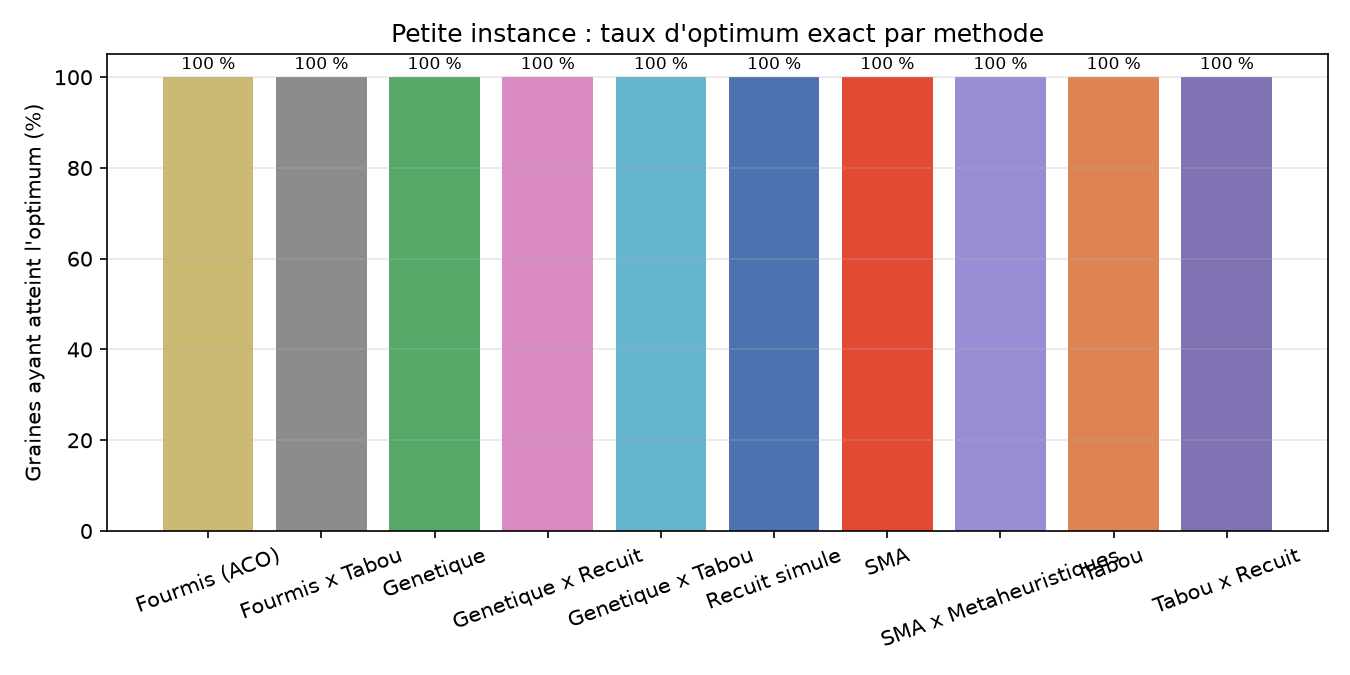
\includegraphics[width=0.92\linewidth,height=0.26\textheight,keepaspectratio]{petite_taux_optimum.png}
    \end{column}
    \begin{column}{0.48\textwidth}
      \begin{alertblock}{La limite}
        \footnotesize Le planning obtenu est optimal \textbf{pour les durées
        prévues}. Dès qu'une urgence arrive, qu'un patient annule, qu'un lit
        ferme ou qu'un bloc prend du retard, l'optimum statique n'est plus le
        bon planning.
      \end{alertblock}
      \begin{block}{Conséquence}
        \footnotesize Il faut passer d'un planning \textbf{optimal} à un
        planning \textbf{robuste}, capable d'absorber les aléas.
      \end{block}
    \end{column}
  \end{columns}
  \source{Instance de validation à 7 patients ; l'optimum exact sert de test de
    correction, pas de départage entre méthodes.}
\end{frame}


% =============================================================================
\section{Approche hybride}
% =============================================================================

% Hybridation : exploration + intensification.
\begin{frame}{Hybridation : combiner exploration et intensification}
  \footnotesize
  \begin{columns}[T,onlytextwidth]
    \begin{column}{0.52\textwidth}
      \begin{block}{Hybrides de métaheuristiques}
        \begin{itemize}
          \item \textbf{Tabou $\times$ Recuit} : voisinage tabou + acceptation
            de Metropolis.
          \item \textbf{Génétique $\times$ Tabou} : recherche tabou courte sur
            le meilleur individu (stratégie lamarckienne).
          \item \textbf{Génétique $\times$ Recuit} : recuit court sur le
            meilleur individu.
          \item \textbf{Fourmis $\times$ Tabou} : intensification de la
            meilleure fourmi.
        \end{itemize}
      \end{block}
    \end{column}
    \begin{column}{0.46\textwidth}
      \begin{exampleblock}{Principe}
        \footnotesize
        \begin{itemize}
          \item une méthode \textbf{globale} explore largement (AG, ACO) ;
          \item une méthode \textbf{locale} intensifie les bonnes zones
            (Tabou, Recuit) ;
          \item l'intensification corrige la faible pression de sélection du
            génétique.
        \end{itemize}
      \end{exampleblock}
      \begin{alertblock}{Apport mesuré}
        \footnotesize Génétique $\times$ Tabou : écart du génétique divisé par
        $\sim$$10^4$ ; Fourmis $\times$ Tabou : écart ACO divisé par
        $\sim$1,7.
      \end{alertblock}
    \end{column}
  \end{columns}
  \source{Distinct de l'hybride d'origine Tabou $\times$ Recuit ; les trois
    autres hybrides ont été construits pour ce projet.}
\end{frame}

% SMA Mesa : architecture de coopération.
\begin{frame}{Système multi-agents : tableau noir et coordination}
  \footnotesize
  \begin{columns}[T,onlytextwidth]
    \begin{column}{0.52\textwidth}
      \centering
      \begin{tikzpicture}[
        ag/.style={draw=mcmExample,rounded corners=2pt,fill=mcmExample!12,
                   minimum height=0.68cm,minimum width=2.35cm,align=center,font=\scriptsize},
        bb/.style={draw=mcmPrimary,rounded corners=2pt,fill=mcmPrimaryMuted,
                   minimum height=1.45cm,minimum width=2.7cm,align=center,font=\scriptsize,thick},
        co/.style={draw=mcmAlert,rounded corners=2pt,fill=mcmAlert!12,
                   minimum height=0.75cm,minimum width=2.7cm,align=center,font=\scriptsize,thick},
        flow/.style={-{Latex},thick,draw=mcmPrimary}]
        \node[ag] (a1) {Agent recuit};
        \node[ag,below=0.28cm of a1] (a2) {Agent tabou};
        \node[ag,below=0.28cm of a2] (a3) {Agent génétique};
        \node[bb,right=1.0cm of a2] (bb) {\textbf{Tableau noir}\\[2pt]meilleure\\solution versionnée};
        \node[co,above=0.35cm of bb] (co) {\textbf{Coordinateur}};
        \draw[flow] (a1.east) -- (bb.west|-a1);
        \draw[flow] (a2) -- (bb);
        \draw[flow] (a3.east) -- (bb.west|-a3);
        \draw[flow,draw=mcmAlert] (co) -- (bb);
      \end{tikzpicture}
    \end{column}
    \begin{column}{0.46\textwidth}
      \begin{block}{Les briques}
        \footnotesize
        \begin{itemize}
          \item \textbf{Tableau noir} : meilleure solution partagée,
            versionnée.
          \item \textbf{Agents} : une stratégie chacun, travaillant par
            \textbf{quanta}.
          \item \textbf{Coordinateur} : migration du meilleur ; redémarrage
            si la version stagne.
        \end{itemize}
      \end{block}
      \begin{exampleblock}{Déterminisme}
        \footnotesize Générateur aléatoire propre à chaque agent : résultats
        reproductibles par graine.
      \end{exampleblock}
    \end{column}
  \end{columns}
  \source{Implémentation Mesa 3.5 : deux SMA (agents simples et agents
    métaheuristiques) coopérant par tableau noir.}
\end{frame}

% Benchmark grande échelle.
\begin{frame}{Benchmark à budget égal : 300 patients, 80 vacations}
  \small
  \begin{columns}[T,onlytextwidth]
    \begin{column}{0.54\textwidth}
      \centering
      \renewcommand{\arraystretch}{1.12}
      \footnotesize
      \begin{tabular}{lrrr}
        \toprule
        Méthode & Écart moyen & Rang & IQR \\
        \midrule
        Recuit simulé      & \textbf{0,015} & \textbf{1,25} & 0,008 \\
        Tabou $\times$ Recuit & \textbf{0,018} & 1,75 & 0,013 \\
        Tabou              & 0,240 & 3,55 & 0,070 \\
        Génétique $\times$ Tabou & 0,261 & 3,75 & 0,106 \\
        SMA                & 1,078 & 5,05 & 0,194 \\
        SMA $\times$ Méta  & 1,196 & 6,15 & 0,154 \\
        Génétique $\times$ Recuit & 2,031 & 6,50 & 0,323 \\
        Fourmis $\times$ Tabou & 1\,006,0 & 8,00 & 180,9 \\
        Fourmis (ACO)      & 2\,031,2 & 9,00 & 256,1 \\
        Génétique          & 2\,836,2 & 10,00 & 380,1 \\
        \bottomrule
      \end{tabular}
    \end{column}
    \begin{column}{0.44\textwidth}
      \centering
      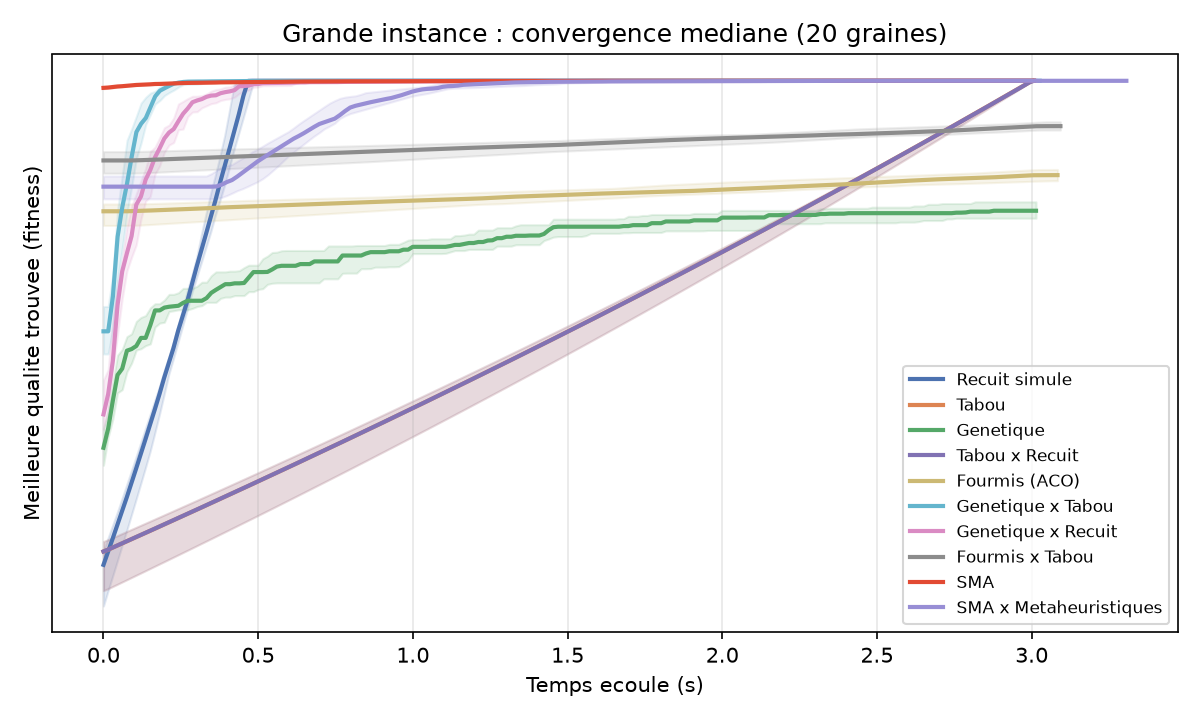
\includegraphics[width=\linewidth,height=0.30\textheight,keepaspectratio]{grande_convergence.png}\\[2pt]
      {\tiny\color{mcmPrimary}\textbf{Convergence médiane} (20 graines, 3 s).}\\[4pt]
      \begin{alertblock}{Lecture}
        \footnotesize Le recuit et Tabou $\times$ Recuit dominent : écarts
        $<0{,}02$ sur une référence de $\sim$38\,800. ACO et génétique
        décrochent (forte variabilité).
      \end{alertblock}
    \end{column}
  \end{columns}
  \source{20 graines, budget 3 s, référence $-38\,847{,}195$ ; écart à la
    meilleure solution observée.}
\end{frame}

% Benchmark échelle réelle.
\begin{frame}{Échelle réelle : 582 patients, 280 vacations}
  \small
  \begin{columns}[T,onlytextwidth]
    \begin{column}{0.5\textwidth}
      \renewcommand{\arraystretch}{1.2}
      \footnotesize
      \begin{tabular}{lrr}
        \toprule
        Méthode & Médiane & Rang moyen \\
        \midrule
        Recuit simulé      & $-16{,}3$ & 1,85 \\
        Tabou $\times$ Recuit & $-14{,}9$ & 2,05 \\
        Tabou              & $-16{,}4$ & 2,65 \\
        Génétique $\times$ Tabou & $-23{,}9$ & 3,50 \\
        SMA                & $-91{,}8$ & 5,85 \\
        Fourmis (ACO)      & $-3\,438{,}8$ & 9,70 \\
        \bottomrule
      \end{tabular}
      \\[4pt]
      {\tiny 20 graines ; référence $-8{,}783$.}
    \end{column}
    \begin{column}{0.48\textwidth}
      \centering
      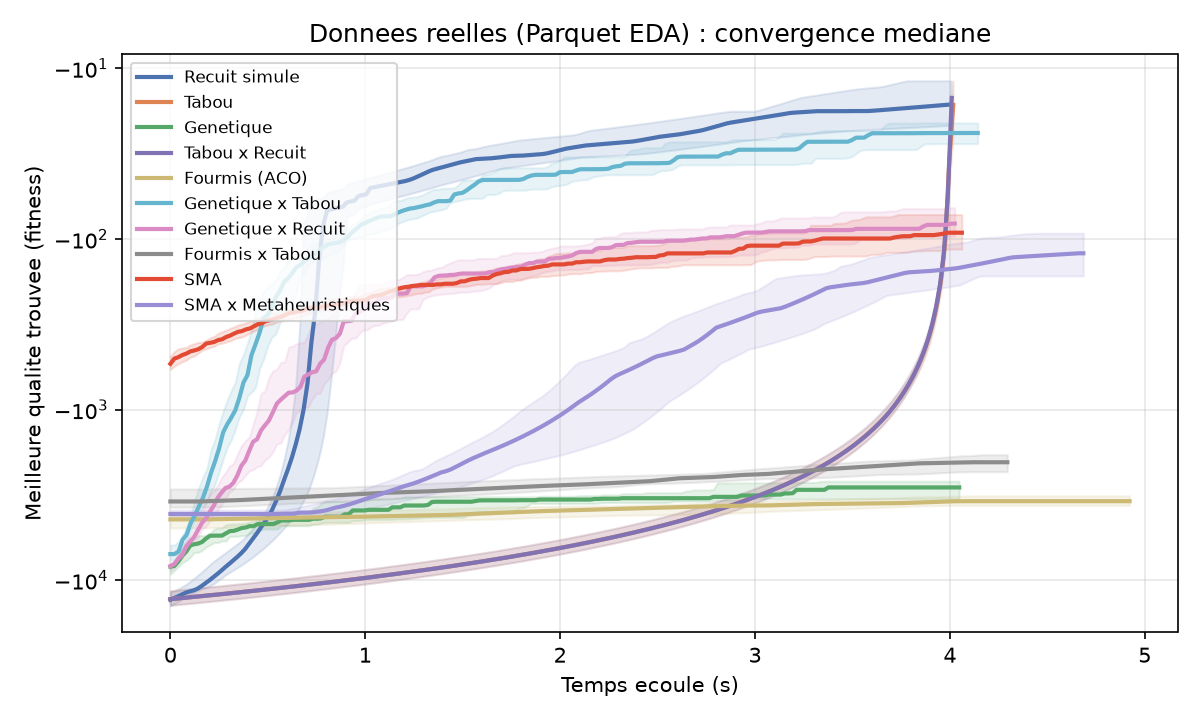
\includegraphics[width=\linewidth,height=0.27\textheight,keepaspectratio]{reelle_convergence.png}\\[2pt]
      \begin{alertblock}{Un couloir faisable étroit}
        \footnotesize La meilleure solution est faisable
        ($\text{violations} = (0,0)$, lits à 42/42). Les méthodes qui
        \textbf{acceptent des dégradations} longent cette frontière ; les
        constructions gloutonnes échouent.
      \end{alertblock}
    \end{column}
  \end{columns}
  \source{Parquet EDA prétraité (40 jours, capacité 600 min/vacation), 4 s par
    méthode et par graine.}
\end{frame}


% =============================================================================
\section{Prise en compte des aléas}
% =============================================================================

% Les quatre aléas.
\begin{frame}{Quatre types d'aléas à absorber}
  \small
  \renewcommand{\arraystretch}{1.3}
  \begin{tabular}{p{3.0cm}p{5.3cm}p{4.5cm}}
    \toprule
    \textbf{Aléa} & \textbf{Description} & \textbf{Impact opérationnel} \\
    \midrule
    Urgence & Patient imprévu, fenêtre temporelle imposée
      & À insérer dans une vacation compatible du jour \\
    Annulation & Patient programmé qui annule
      & Libère un créneau \textbf{et} des lits \\
    Indisponibilité lits & Réduction de capacité sur
      $[j_{\text{début}}, j_{\text{fin}}]$
      & Force la réaffectation des séjours chevauchants \\
    Retard bloc & Prolongation ou incident sur une vacation
      & Ampute la capacité utile disponible \\
    \bottomrule
  \end{tabular}

  \vspace{0.3cm}
  \begin{alertblock}{Deux réponses complémentaires}
    \small \textbf{Proactive} : générer des plannings alternatifs robustes.
    \textbf{Réactive} : adapter dynamiquement sous contrainte de stabilité.
  \end{alertblock}
  \source{Chaque aléa est modélisé par une classe dédiée et un simulateur
    reproductible (\texttt{generer\_scenario\_aleas}).}
\end{frame}

% Proactif : plannings alternatifs.
\begin{frame}{Proactif : plannings alternatifs et double proposition}
  \small
  \begin{columns}[T,onlytextwidth]
    \begin{column}{0.5\textwidth}
      \begin{block}{Quatre profils de planning}
        \begin{itemize}
          \item \textbf{Nominal} : optimal à 100\,\% de la capacité.
          \item \textbf{Robuste bufferisé} : réserve de capacité bloc
            ($\sim$15\,\%) et lits pour absorber les imprévus.
          \item \textbf{Sécurité lits} : lissage strict, sous-saturation pour
            parer aux fermetures.
          \item \textbf{Alternatif Date B} : haute qualité, diversifié par
            rapport au nominal.
        \end{itemize}
      \end{block}
    \end{column}
    \begin{column}{0.48\textwidth}
      \begin{exampleblock}{Double proposition chirurgicale}
        \footnotesize Pour chaque patient, la table
        \texttt{extraire\_options\_date\_a\_b} produit :
        \begin{center}
          \textbf{Date A} (optimale) \quad / \quad \textbf{Date B}
          (alternative)
        \end{center}
        Le praticien choisit en connaissance des tensions sur les lits et le
        bloc.
      \end{exampleblock}
      \begin{alertblock}{Objectif}
        \footnotesize Passer d'un planning \textbf{optimal} à un planning
        \textbf{robuste} : ne pas casser tout le programme parce qu'un imprévu
        survient.
      \end{alertblock}
    \end{column}
  \end{columns}
  \source{Aperçu : un buffer de capacité réduit la qualité nominale mais
    absorbe les aléas sans décaler les patients.}
\end{frame}

% Réactif : adaptation dynamique.
\begin{frame}{Réactif : adaptation sous contrainte de stabilité}
  \small
  \begin{columns}[T,onlytextwidth]
    \begin{column}{0.52\textwidth}
      \begin{block}{Trois garde-fous}
        \begin{itemize}
          \item \textbf{Gel du passé} : tout acte antérieur au jour courant est
            sanctuarisé.
          \item \textbf{Insertion prioritaire des urgences} dans leur fenêtre
            clinique.
          \item \textbf{Moindre perturbation} : on minimise les déplacements de
            patients futurs.
        \end{itemize}
      \end{block}
    \end{column}
    \begin{column}{0.46\textwidth}
      \begin{alertblock}{Score d'adaptation}
        \footnotesize
        \[
          \begin{aligned}
            \text{Score} = \text{Fitness} &- w_p \cdot \text{Déplacements} \\
                                          &- w_j \cdot \text{Changements de jour}
          \end{aligned}
        \]
        Le planning reste proche de celui annoncé aux patients.
      \end{alertblock}
      \begin{exampleblock}{Rapport d'arbitrage}
        \footnotesize Synthèse chiffrée des motifs de chaque déplacement et des
        urgences accueillies.
      \end{exampleblock}
    \end{column}
  \end{columns}
  \source{Rapport produit automatiquement par \texttt{adapter\_planning} pour
    garder la décision explicable.}
\end{frame}

% Resultat 1 : plan fige ou replanification (repris de Kaua_SMA_9_octobre.tex).
\begin{frame}{Résultats : plan figé ou replanification ?}
  \small
  \vspace{0.15cm}
  \centering
  \renewcommand{\arraystretch}{1.32}
  \setlength{\tabcolsep}{8pt}
  \begin{tabular}{llrr}
    \toprule
    Situation & Politique & Terminées / 279 & Dépassement (min) \\
    \midrule
    Sans fermeture & Figée ou réactive & 262 & 2\,954 \\
    \midrule
    Avec fermeture & Figée & \textbf{255} & 2\,911 \\
    Avec fermeture & Réactive & 251 & \textbf{2\,716} \\
    \bottomrule
  \end{tabular}
  \vspace{0.35cm}
  \begin{alertblock}{Compromis observé, pas un gain systématique}
    \small La replanification réduit le dépassement de \textbf{195 min}
    mais termine \textbf{4 interventions de moins} sur cette fenêtre.
  \end{alertblock}
  \source{Modèle prédictif, planificateur glouton, 42 lits synthétiques, 2 salles, 3--31 janvier 2022, graine 0. Dépassement = occupation + remise en état après 17h.}
\end{frame}


% =============================================================================
\section{Simulations et scénarios réalistes}
% =============================================================================

\begin{frame}{Simulation : charges historiques et ressources supposées}
  \small
  \begin{columns}[T,onlytextwidth]
    \begin{column}{0.32\textwidth}
      \begin{block}{Données}
        \centering
        {\Large\bfseries 14\,434}\\
        cas exploitables\\[5pt]
        73 exclusions\\[5pt]
        2019--2021 : estimation\\
        2022 : exécution cachée
      \end{block}
    \end{column}
    \begin{column}{0.32\textwidth}
      \begin{block}{Deux charges}
        \centering
        {\Large\bfseries 58} cas / 5 jours\\[5pt]
        {\Large\bfseries 279} cas / 22 jours\\[5pt]
        Cohorte test 2022\\
        Patients hors entraînement
      \end{block}
    \end{column}
    \begin{column}{0.32\textwidth}
      \begin{block}{Scénarios}
        \centering
        2 salles, 08h--17h\\
        15 min de remise en état\\[5pt]
        42 ou 10 lits \textbf{synthétiques}\\
        Salle 1 fermée de 10h à 12h
      \end{block}
    \end{column}
  \end{columns}
  \vspace{0.23cm}
  \begin{exampleblock}{Comparaison appariée}
    \small Mêmes arrivées, mêmes durées réellement observées, mêmes
    ressources. Trois informations : médianes, prédictions ML, oracle.
  \end{exampleblock}
  \source{Fenêtres du 3 au 7 et du 3 au 31 janvier 2022 ; charges de travail, pas preuve de passage à l'échelle des solveurs.}
\end{frame}

\begin{frame}{Intégration SMA : planifier, simuler, corriger}
  \small
  \centering
  \vspace{0.25cm}
  \begin{tikzpicture}[
      card/.style={draw=McmTerracotta,rounded corners=2pt,fill=white,
                   minimum height=2.05cm,text width=3.10cm,align=center,
                   inner sep=5pt,font=\small},
      flow/.style={-{Latex[length=2.5mm]},thick,draw=McmTerracotta}]
    \node[card] (input) at (0,0) {\textbf{Entrées disponibles}\\[3pt]
      Interventions à programmer\\Durées prévues : salle et séjour restant};
    \node[card] (solver) at (4.15,0) {\textbf{Planificateur}\\[3pt]
      Glouton ou métaheuristique\\Planning proposé puis validé};
    \node[card] (mesa) at (8.30,0) {\textbf{Exécution Mesa}\\[3pt]
      Agents-épisodes\\Salles à la minute, lits sur plusieurs jours};
    \draw[flow] (input) -- (solver);
    \draw[flow] (solver) -- (mesa);
    \draw[flow] (mesa.south) -- ++(0,-0.80) -| (solver.south);
    \node[font=\scriptsize,text=McmMuted,fill=McmWarm,inner sep=2pt]
      at (6.22,-1.53) {Observations et replanification des cas en attente};
  \end{tikzpicture}
  \vspace{0.23cm}

  \begin{exampleblock}{Le rôle du SMA ici}
    \small Le solveur utilise des durées estimées. Mesa révèle les résultats
    réels au coordinateur.
  \end{exampleblock}
  \source{Implémenté : hospital\_sim (Mesa 3.5.1). Les lits sont des ressources ; l'ambulatoire reste à intégrer.}
\end{frame}

\begin{frame}{Simulation dynamique : fermeture temporaire d'une salle}
  \small
  \centering
  \begin{tikzpicture}[x=1.0cm,y=1cm,>=Latex]
    \draw[very thick,draw=McmInk] (0,0) -- (10.3,0);
    \draw[line width=4pt,draw=McmAmber] (2.3,0) -- (5.5,0);
    \foreach \x/\lab in {0/08h,2.3/10h,5.5/12h,10.3/17h} {
      \draw[draw=McmInk] (\x,-0.12) -- (\x,0.12);
      \node[below=5pt,font=\scriptsize] at (\x,0) {\lab};
    }
    \node[above=8pt,text=McmAmber,font=\small\bfseries] at (3.9,0)
      {Salle 1 : aucune nouvelle entrée};
  \end{tikzpicture}
  \vspace{0.45cm}
  \begin{columns}[T,onlytextwidth]
    \begin{column}{0.49\textwidth}
      \begin{block}{Plan figé}
        \small Affectations et ordre initiaux conservés.
        Les cas suivants attendent que la salle soit disponible.
      \end{block}
    \end{column}
    \begin{column}{0.49\textwidth}
      \begin{exampleblock}{Plan réactif}
        \small Aux changements 10h/12h, le coordinateur soumet un
        nouveau planning pour les \textbf{cas en attente}.
      \end{exampleblock}
    \end{column}
  \end{columns}
  \vspace{0.10cm}
  \centering\small Intervention déjà commencée : elle se termine normalement.
  Proposition invalide : ancien plan conservé, garde d'exécution active.
  \source{Urgences, annulations et indisponibilités de lits ne sont pas encore des aléas exécutés dans ce simulateur.}
\end{frame}

\begin{frame}{Simulations : du planning à l'exécution}
  \footnotesize
\textbf{Une question commune : utiliser le bloc sans saturer les lits.}
\par\vspace{1.5mm}
\centering
\renewcommand{\arraystretch}{1.18}
\setlength{\tabcolsep}{5pt}
\begin{tabular}{@{}lp{3.15cm}p{6.25cm}@{}}
\toprule
\textbf{Évaluation} & \textbf{Population} & \textbf{Protocole}\\\midrule
Recherche statique & 300 patients / 80 vacations & 20 graines ; même budget de 3 s par méthode\\
Échelle historique & 582 patients / 280 vacations & 40 jours ; 4 s par méthode\\
Exécution simulée & 279 interventions / 22 jours & 2 salles, 08h--17h ; 42 ou 10 lits synthétiques\\
Incertitude LOS & 420 patients / 30 jours & 42 lits ; 10 graines ; 200 scénarios par planning\\\bottomrule
\end{tabular}
\vspace{0.05cm}
\begin{columns}[T,onlytextwidth]
\begin{column}{.49\textwidth}
\begin{block}{Évaluation statique}
Comparer la qualité des plannings à ressources et budget identiques.
\end{block}
\end{column}
\begin{column}{.49\textwidth}
\begin{exampleblock}{Exécution simulée}
Observer les interventions terminées, les dépassements et l'occupation des lits.
\end{exampleblock}
\end{column}
\end{columns}
\end{frame}

\begin{frame}{Scénarios : prévoir, puis confronter au réel}
  \footnotesize
\begin{block}{Du scénario à l'évaluation}
\centering
\textbf{Durées disponibles} (salle et séjour estimés)
$\longrightarrow$
\textbf{Planning} (bloc et lits)
$\longrightarrow$
\textbf{Évaluation} (exécution ou scénarios LOS)
\end{block}
\vspace{0.08cm}
\begin{columns}[T,onlytextwidth]
\begin{column}{.48\textwidth}
\begin{block}{Exécution historique : simulation SMA}
\textbf{Mêmes arrivées et durées observées.}\\
Médianes, prédictions ML ou oracle.\\
Salle 1 fermée de \textbf{10h à 12h} ; plan figé ou replanification des cas en attente.\\
Les actes commencés se terminent normalement.
\end{block}
\end{column}
\begin{column}{.48\textwidth}
\begin{block}{Séjours incertains : Monte Carlo LOS}
Planifier avec la prédiction ponctuelle ou la \textbf{borne haute conformelle}.\\
Planning figé ; \textbf{200 scénarios}, tirages communs.\\
Perturbation uniforme $\pm1{,}02$ jour, arrondie ; plancher d'un jour.\\
Un séjour prolongé mobilise davantage de lits.
\end{block}
\end{column}
\end{columns}
\end{frame}
% =============================================================================
\section{Résultats et comparaisons}
% =============================================================================

\begin{frame}{Statique vs hybride : la hiérarchie confirmée}
  \footnotesize
  \begin{columns}[T,onlytextwidth]
    \begin{column}{0.52\textwidth}
      \begin{block}{À budget temps égal}
        \begin{itemize}
          \item Recuit simulé $\approx$ Tabou $\times$ Recuit (tête) ;
          \item puis Tabou $\approx$ Génétique $\times$ Tabou ;
          \item SMA au milieu, freinés par le coût de coordination ;
          \item ACO et génétique distancés, surtout à l'échelle réelle.
        \end{itemize}
      \end{block}
      \begin{exampleblock}{Le message}
        \footnotesize Les \textbf{hybrides} apportent un gain net
        (Génétique $\times$ Tabou, Fourmis $\times$ Tabou) ; les méthodes
        \textbf{locales} restent les plus fiables sur un paysage rugueux.
      \end{exampleblock}
    \end{column}
    \begin{column}{0.46\textwidth}
      \centering
      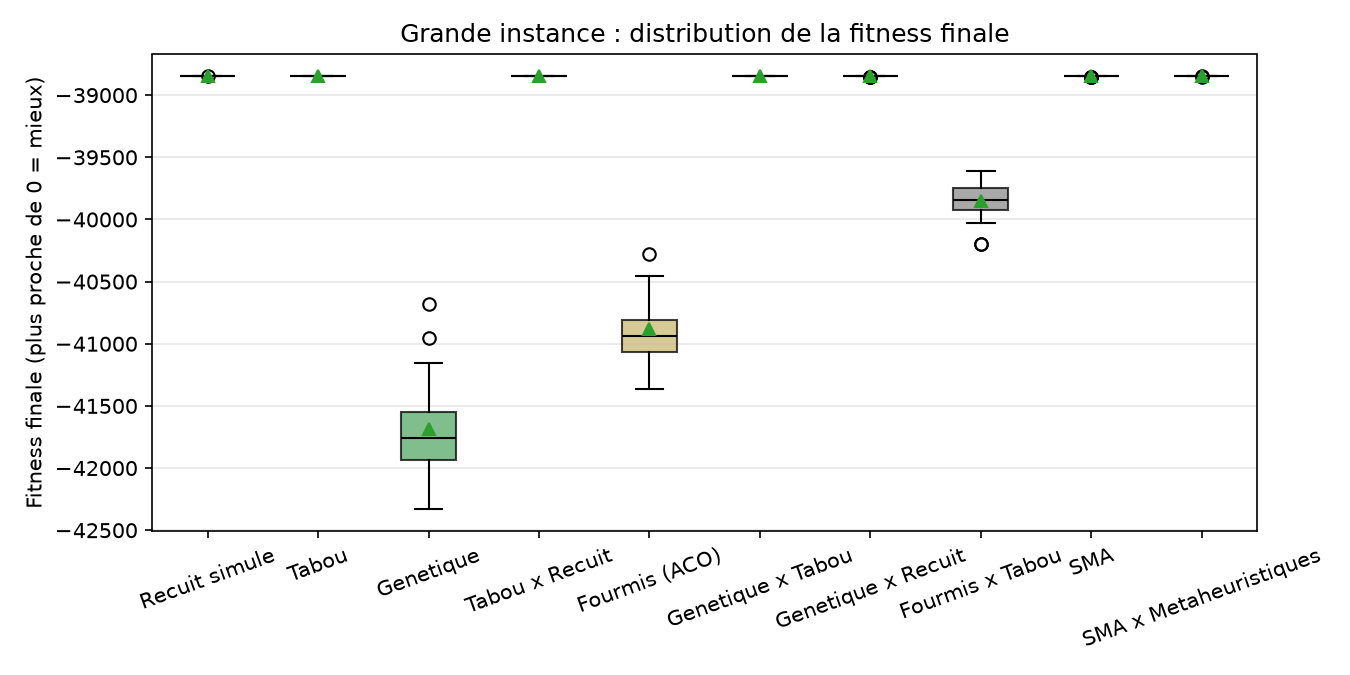
\includegraphics[width=\linewidth,height=0.28\textheight,keepaspectratio]{grande_boxplot.png}\\[2pt]
      {\tiny\color{mcmPrimary}\textbf{Dispersion} de la fitness finale
        (grande échelle).}\\[4pt]
      \begin{alertblock}{Fiabilité}
        \footnotesize 10/10 méthodes atteignent l'optimum exact en petite
        instance ; aucune ne viole les contraintes dures.
      \end{alertblock}
    \end{column}
  \end{columns}
  \source{Synthèse des campagnes 20 graines : petite (7), grande (300) et réelle
    (582) instances.}
\end{frame}

\begin{frame}{Résultats : prédictions, oracle et capacité}
  \small
  \centering
  \renewcommand{\arraystretch}{1.40}
  \setlength{\tabcolsep}{11pt}
  \begin{tabular}{lrrr}
    \toprule
    Capacité & Médianes & Modèle & Oracle \\
    \midrule
    42 lits & 246 & \textbf{251} & 260 \\
    10 lits & \textbf{111} & 108 & 115 \\
    \bottomrule
  \end{tabular}
  \vspace{0.38cm}
  \begin{columns}[T,onlytextwidth]
    \begin{column}{0.49\textwidth}
      \begin{block}{42 lits : non saturés}
        \small Au plus 30 lits occupés en fin de journée.
        Le modèle gagne 5 cas sur les médianes, mais reste
        9 cas derrière l'oracle.
      \end{block}
    \end{column}
    \begin{column}{0.49\textwidth}
      \begin{alertblock}{10 lits : saturation}
        \small Les 10 lits sont occupés en fin de journée
        sur \textbf{21 des 22 jours} opératoires.
      \end{alertblock}
    \end{column}
  \end{columns}
  \source{Cas terminés sur 279 ; politique réactive, fermeture 10h--12h, 2 salles, graine 0. Oracle = durées futures révélées, pas optimum garanti.}
\end{frame}

\begin{frame}{Résultats : mieux chercher, mieux informer}
  \footnotesize
\begin{columns}[T,onlytextwidth]
\begin{column}{.48\textwidth}
\textbf{Choix de la méthode : budget identique}\par
300 patients / 80 vacations ; 3 s ; 20 graines.
\par\vspace{0.8mm}
\centering
\renewcommand{\arraystretch}{1.1}
\begin{tabular}{@{}lr@{}}
\toprule
Méthode & Écart moyen\\\midrule
\textbf{Recuit simulé} & \textbf{0,015}\\
\textbf{Tabou $\times$ Recuit} & \textbf{0,018}\\
Tabou & 0,240\\
Génétique $\times$ Tabou & 0,261\\\bottomrule
\end{tabular}
\par\vspace{0.5mm}
\raggedright
Écart à la meilleure solution observée,\newline pas à un optimum prouvé.
\par\vspace{0.5mm}
\textbf{582 / 280 :} même groupe de tête ; meilleure solution faisable, lits à 42/42.
\end{column}
\begin{column}{.48\textwidth}
\textbf{Qualité de l'information : mêmes ressources}\par
279 interventions ; 42 lits ; fermeture ; réactif.
\par\vspace{0.8mm}
\centering
\renewcommand{\arraystretch}{1.1}
\begin{tabular}{@{}lr@{}}
\toprule
Information & Terminées / 279\\\midrule
Médianes & 246\\
\textbf{Prédictions ML} & \textbf{251}\\
Oracle & 260\\\bottomrule
\end{tabular}
\par\vspace{0.5mm}
\raggedright
\textbf{ML : +5 interventions} par rapport aux médianes ; 9 de moins que l'oracle.
\par\vspace{0.5mm}
À \textbf{10 lits}, médianes 111 / ML 108 : le gain dépend des ressources.
\end{column}
\end{columns}
\vspace{0.5mm}
\centering
{\color{McmTerracotta}\bfseries Recuit et Tabou $\times$ Recuit en tête ;
la prédiction aide, sans gain systématique.}
\end{frame}

\begin{frame}{Aléas : deux compromis opérationnels}
  \footnotesize
\begin{columns}[T,onlytextwidth]
\begin{column}{.45\textwidth}
\textbf{Fermeture du bloc : adapter l'exécution}\par
279 interventions ; ML ; 42 lits ; salle fermée 10h--12h.
\par\vspace{0.8mm}
\centering
\renewcommand{\arraystretch}{1.1}
\begin{tabular}{@{}lrr@{}}
\toprule
Plan & Terminées & Dépass. (min)\\\midrule
Figé & 255 & 2\,911\\
Réactif & 251 & 2\,716\\\bottomrule
\end{tabular}
\par\vspace{0.8mm}
\raggedright
{\color{McmTerracotta}\bfseries $-195$ min de dépassement,\\mais 4 interventions de moins.}
\par\vspace{0.5mm}
Dépassement : occupation et remise en état après 17h.
\end{column}
\begin{column}{.52\textwidth}
\textbf{LOS : anticiper les séjours longs}\par
420 patients / 30 jours ; 42 lits ; Monte Carlo.
\par\vspace{0.8mm}
\centering
\renewcommand{\arraystretch}{1.1}
\setlength{\tabcolsep}{4pt}
\begin{tabular}{@{}lrr@{}}
\toprule
 & Dégradation & Coût moyen\\
 & \multicolumn{2}{c}{Ponctuel $\rightarrow$ borne haute}\\\midrule
Recuit & $109\rightarrow13$ & $5\,316\rightarrow5\,384$\\
Tabou & $115\rightarrow17$ & $5\,313\rightarrow5\,376$\\
Tabou $\times$ Recuit & $112\rightarrow6$ & $5\,311\rightarrow5\,413$\\\bottomrule
\end{tabular}
\par\vspace{0.8mm}
\raggedright
{\color{McmTerracotta}\bfseries Moins de dégradation,\\mais un coût moyen plus élevé.}
\par\vspace{0.5mm}
Dégradation : $\mathbb E[C]-C_{\mathrm{ponctuel}}$\newline pour le \textbf{même} planning.
\end{column}
\end{columns}
\vspace{0.5mm}
\centering
{\color{McmTerracotta}\bfseries La robustesse a un prix :
choisir le compromis, sans gain universel.}
\end{frame}
% =============================================================================
\section{L'application KYST}
% =============================================================================
% KYST (Keep Your Surgeries Timelies) : l'outil web qui met le flux tiré entre
% les mains des équipes. Sources : interface/docs (Features.md, Frontend.md),
% interface/ansible/roles/kyst, docs/todo.md.

% Ouverture : l'application est en ligne, le jury peut l'ouvrir pendant la soutenance.
\begin{frame}{KYST est en ligne}
  \begin{columns}[c,onlytextwidth]
    \begin{column}{0.56\textwidth}
      {\Large\bfseries\color{mcmPrimary} sandbox.rezoleo.fr}\\[0.3cm]
      \small
      KYST (\emph{Keep Your Surgeries Timelies}) est l'application web du
      projet. Elle est \textbf{déployée et utilisable dès maintenant}, sur
      ordinateur comme sur téléphone.
      \vspace{0.15cm}
      \begin{exampleblock}{Ce que l'on peut y faire}
        \begin{itemize}
          \item saisir une demande d'intervention en consultation ;
          \item obtenir deux dates, \textbf{justifiées}, compatibles avec le
            bloc et les lits ;
          \item confirmer une date : la vacation et le lit sont réservés.
        \end{itemize}
      \end{exampleblock}
    \end{column}
    \begin{column}{0.40\textwidth}
      \centering
      \qrcode[height=4.2cm]{https://sandbox.rezoleo.fr}\\[0.2cm]
      {\footnotesize Données de démonstration\\synthétiques, aucune donnée réelle}
    \end{column}
  \end{columns}
\end{frame}

% Architecture : trois services, le navigateur ne parle qu'au front.
\begin{frame}{Architecture}
  \small
  \centering
  \begin{tikzpicture}[
      card/.style={draw=McmTerracotta,rounded corners=2pt,fill=white,
                   minimum height=1.25cm,text width=2.0cm,align=center,
                   inner sep=3pt,font=\footnotesize},
      ext/.style={card,draw=McmMuted,dashed},
      flow/.style={{Latex[length=2mm]}-{Latex[length=2mm]},thick,draw=McmTerracotta},
      lab/.style={font=\scriptsize,text=McmMuted,inner sep=1pt}]
    \node[ext]  (user)  at (0,0)    {\textbf{Navigateur}\\ordinateur\\ou téléphone};
    \node[card] (front) at (3.5,0)  {\textbf{Front}\\SvelteKit};
    \node[card] (api)   at (7.0,0)  {\textbf{API}\\FastAPI};
    \node[card] (db)    at (10.5,0) {\textbf{Base}\\PostgreSQL};
    \node[ext]  (ai)    at (7.0,-1.85) {\textbf{Modules IA}\\prédictions,\\ordonnanceur};
    \draw[flow] (user)  -- node[lab,above=3pt] {HTTPS} (front);
    \draw[flow] (front) -- node[lab,above=3pt] {interne} (api);
    \draw[flow] (api)   -- node[lab,above=3pt] {SQL} (db);
    \draw[flow] (api)   -- node[lab,right=3pt] {contrats Python} (ai);
    \begin{scope}[on background layer]
      \node[draw=McmSage,dashed,rounded corners=3pt,inner sep=5pt,
            fit=(front)(api)(db)(ai)] (srv) {};
    \end{scope}
    \node[font=\scriptsize,text=McmSage,anchor=south east] at ([shift={(0,1pt)}]srv.north east)
      {serveur : Podman rootless, Ansible};
  \end{tikzpicture}
  \vspace{0.05cm}
  \begin{columns}[T,onlytextwidth]
    \begin{column}{0.49\textwidth}
      \begin{block}{Séparation des rôles}
        \footnotesize Le navigateur n'appelle \textbf{jamais l'API} : seul le
        serveur du front lui parle. L'API reste l'unique autorité sur les
        droits et les données.
      \end{block}
    \end{column}
    \begin{column}{0.49\textwidth}
      \begin{exampleblock}{Point de branchement de l'IA}
        \footnotesize Les modèles et le solveur se branchent derrière des
        \textbf{interfaces fixes}, sans modifier l'application.
      \end{exampleblock}
    \end{column}
  \end{columns}
\end{frame}

% Interface : le parcours principal, de la consultation à la sortie.
\begin{frame}{Interface : de la consultation à la sortie}
  \small
  \centering
  \begin{tikzpicture}[
      stage/.style={draw=McmTerracotta,rounded corners=2pt,fill=white,
                   minimum height=1.25cm,text width=2.05cm,align=center,
                   inner sep=3pt,font=\scriptsize},
      human/.style={stage,fill=McmSand},
      flow/.style={-{Latex[length=2mm]},thick,draw=McmTerracotta}]
    \node[human] (s1) at (0,0)     {\textbf{Demande}\\saisie en\\consultation};
    \node[stage]  (s2) at (2.75,0)  {\textbf{Prédiction}\\temps en salle,\\séjour, hébergement};
    \node[stage]  (s3) at (5.50,0)  {\textbf{Dates A et B}\\chacune avec\\ses raisons};
    \node[human] (s4) at (8.25,0)  {\textbf{Confirmation}\\par le\\chirurgien};
    \node[stage]  (s5) at (11.00,0) {\textbf{Réservation}\\vacation\\et lit};
    \foreach \a/\b in {s1/s2,s2/s3,s3/s4,s4/s5} \draw[flow] (\a) -- (\b);
    \draw[flow] (s4.south) -- ++(0,-0.45) -| node[pos=0.25,below,font=\scriptsize,text=McmMuted]
      {écarte : nouvelles dates} (s3.south);
  \end{tikzpicture}
  \vspace{0.15cm}
  \begin{columns}[T,onlytextwidth]
    \begin{column}{0.49\textwidth}
      \begin{block}{Pages}
        \footnotesize
        \textbf{Tableau de bord} : lits du jour, remplissage du bloc,
        demandes en attente.\\
        \textbf{Bloc} : semaine par salle, jauge de chaque vacation.\\
        \textbf{Lits} : occupation prévue sur 7, 14 ou 28 jours.\\
        \textbf{Ressources} : salles, unités, chirurgiens.
      \end{block}
    \end{column}
    \begin{column}{0.49\textwidth}
      \begin{exampleblock}{Choix d'interface}
        \footnotesize
        \begin{itemize}
          \item Le chirurgien \textbf{garde la décision} : rien n'est
            programmé sans confirmation.
          \item Jours tendus signalés par un symbole, pas seulement la
            couleur.
          \item Utilisable sur téléphone, en consultation.
        \end{itemize}
      \end{exampleblock}
    \end{column}
  \end{columns}
  \source{En beige : étapes humaines. Le chirurgien peut aussi relancer le
    calcul ou annuler ; la place est alors libérée.}
\end{frame}

% Fonctionnalités : état réel par rapport au cahier des charges.
\begin{frame}{Fonctionnalités et cahier des charges}
  \footnotesize
  \centering
  \renewcommand{\arraystretch}{1.18}
  \setlength{\tabcolsep}{7pt}
  \begin{tabular}{p{6.6cm}p{5.6cm}l}
    \toprule
    Attendu & Dans KYST & État \\
    \midrule
    Donner une date au patient en consultation & Saisie et dates A/B, sur
      mobile & {\color{McmSage}\textbf{Disponible}} \\
    Prédire séjour, temps opératoire, hébergement & Prédictions avec
      intervalles & {\color{McmAmber}\textbf{Démo}} \\
    Proposer une ou deux dates selon bloc et lits & Vérifiées et justifiées
      & {\color{McmAmber}\textbf{Démo}} \\
    Marge pour les urgences & 10\,\% de chaque vacation réservés &
      {\color{McmSage}\textbf{Disponible}} \\
    Suivi du remplissage des lits & Occupation prévue, jours tendus &
      {\color{McmSage}\textbf{Disponible}} \\
    Expliquer, laisser la main au chirurgien & Raisons affichées,
      confirmation & {\color{McmSage}\textbf{Disponible}} \\
    Apprendre de la réalité observée & Durées réelles, précision mesurée &
      {\color{McmSage}\textbf{Disponible}} \\
    Vacations hebdomadaires par spécialité & Ouverture une à une &
      {\color{McmTerracotta}\textbf{Partiel}} \\
    Lissage week-ends et vacances & --- & {\color{McmMuted}\textbf{Prévu}} \\
    \bottomrule
  \end{tabular}
  \source{Démo : le parcours fonctionne de bout en bout, avec des durées de
    démonstration et un ordonnanceur glouton à la place des modèles et du
    solveur.}
\end{frame}

% Sécurité : application, données, infrastructure.
\begin{frame}{Sécurité et confidentialité}
  \footnotesize
  \begin{columns}[T,onlytextwidth]
    \begin{column}{0.32\textwidth}
      \begin{block}{Comptes et sessions}
        \begin{itemize}
          \item Compte validé par un administrateur, \textbf{rôles} vérifiés
            par l'API.
          \item Mots de passe hachés (\textbf{Argon2}), tentatives limitées.
          \item Jetons en cookies \textbf{HttpOnly}, \textbf{Secure},
            invisibles du JavaScript.
          \item Formulaires protégés contre les requêtes intersites (CSRF).
        \end{itemize}
      \end{block}
    \end{column}
    \begin{column}{0.32\textwidth}
      \begin{exampleblock}{Données patient}
        \begin{itemize}
          \item \textbf{Pseudonymisées} : ni nom ni date de naissance, seulement
            l'année et le sexe.
          \item Tableaux de bord \textbf{agrégés}, sans ligne patient.
          \item Chaque décision garde son auteur et sa date.
          \item Aucune donnée réelle dans le dépôt ni sur le serveur.
        \end{itemize}
      \end{exampleblock}
    \end{column}
    \begin{column}{0.32\textwidth}
      \begin{alertblock}{Infrastructure}
        \begin{itemize}
          \item API et base \textbf{non exposées} : pare-feu fermé par défaut.
          \item Seul le reverse proxy TLS joint le front.
          \item Conteneurs \textbf{sans privilèges} (Podman rootless).
          \item Secrets générés au déploiement, hors du dépôt.
        \end{itemize}
      \end{alertblock}
    \end{column}
  \end{columns}
  \source{Prévu : journal d'audit des accès aux données patient, droits limités
    aux demandes de chaque chirurgien.}
\end{frame}

% Reste a faire : d'abord brancher les travaux des autres parties.
\begin{frame}{Ce qui reste à faire}
  \footnotesize
  \begin{columns}[T,onlytextwidth]
    \begin{column}{0.49\textwidth}
      \begin{alertblock}{Brancher l'IA du projet}
        \begin{itemize}
          \item Modèles de \textbf{durée de séjour} et de \textbf{temps en
            salle}, classifieur ambulatoire / conventionnel.
          \item Remplacer l'ordonnanceur glouton par le \textbf{solveur}
            (tabou, recuit, génétique), hors du fil des requêtes.
          \item Relier le coordinateur de \texttt{hospital\_sim} : urgences,
            annulations, salle indisponible.
        \end{itemize}
      \end{alertblock}
    \end{column}
    \begin{column}{0.49\textwidth}
      \begin{block}{Compléter l'outil}
        \begin{itemize}
          \item \textbf{Planning du jour} : ordre de passage et remise en état.
          \item Modèles de vacations hebdomadaires tirés de l'historique.
          \item Aide au lissage des week-ends et vacances.
          \item Droits par chirurgien et journal d'audit.
          \item Migrations de schéma, tests de bout en bout.
        \end{itemize}
      \end{block}
    \end{column}
  \end{columns}
  \vspace{0.05cm}
  \begin{exampleblock}{Message clé}
    \centering
    L'application est prête à \textbf{recevoir les modèles et le solveur} :
    ils remplacent les valeurs de démonstration sans changer l'interface.
  \end{exampleblock}
\end{frame}

% Rappel : la démonstration est accessible maintenant.
\begin{frame}{Essayez KYST}
  \centering
  \vspace{0.2cm}
  \qrcode[height=5.2cm]{https://sandbox.rezoleo.fr}\\[0.45cm]
  {\LARGE\bfseries\color{mcmPrimary} sandbox.rezoleo.fr}\\[0.25cm]
  \small Demandez un accès sur le site : un administrateur de l'équipe le valide.
\end{frame}

% =============================================================================
\section{Conclusion et perspectives}
% =============================================================================

\begin{frame}{Contributions et perspectives}
  \footnotesize
  \begin{columns}[T,onlytextwidth]
    \begin{column}{0.5\textwidth}
      \begin{exampleblock}{Contributions}
        \begin{itemize}
          \item Approche \textbf{conjointe} bloc + lits + ambulatoire, en
            dynamique.
          \item \textbf{Dix méthodes} comparées, validées à l'optimum exact.
          \item \textbf{Aléas} : plannings alternatifs (Date A / Date B) et
            adaptation stable.
          \item Écosystème complet : solveur, simulation Mesa, GUI, CLI.
        \end{itemize}
      \end{exampleblock}
    \end{column}
    \begin{column}{0.48\textwidth}
      \begin{alertblock}{Suite du travail}
        \begin{itemize}
          \item Valider le \textbf{proxy de spécialité} et les poids du coût.
          \item Intégrer l'\textbf{ambulatoire} dans le simulateur Mesa.
          \item Boucle journalière d'indicateurs opérationnels.
          \item Budgets plus longs pour départager le haut du tableau.
        \end{itemize}
      \end{alertblock}
    \end{column}
  \end{columns}

  \vspace{0.15cm}
  \begin{block}{Message clé}
    \centering
    L'originalité du fil rouge est la \textbf{gestion conjointe et coordonnée
    du bloc, des lits et de l'ambulatoire} dans un contexte dynamique.
  \end{block}
\end{frame}

% =============================================================================
% BIBLIOGRAPHIE
% =============================================================================


\nocite{*}
\begin{frame}{Références}
  \footnotesize
  \printbibliography[heading=none]
\end{frame}

% =============================================================================
% CLÔTURE
% =============================================================================
{\setbeamercolor{normal text}{fg=mcmPrimaryFg,bg=mcmPrimary!70}
\begin{frame}[plain,noframenumbering]
  \begin{center}
    \Large
    Merci de votre attention\\[0.5em]
    Questions ?
  \end{center}
\end{frame}
}

\end{document}
